\chapter{Experimental Results}


\section{Evaluation Setup}
All six configurations were evaluated using GPT-4o-mini as the external judge for both RAGAS metrics and the LLM-as-a-Judge scores. Each configuration was run on the same stratified 20-question sample described in Section 5.7.1. Fourteen of the twenty questions were answerable (is\_impossible=False) and six were unanswerable. RAGAS metrics were computed only on the answerable subset; Judge Correctness was also restricted to answerable questions; Judge Conciseness was computed for all non-error answers. Results for each question were written to a timestamped CSV file and averaged per configuration. The six unanswerable questions were evaluated manually: for each one, the model's response was inspected to determine whether it correctly acknowledged that the requested information was not present in the contract. A response was counted as correct if it explicitly stated that the answer could not be found, without fabricating a plausible-sounding but unsupported answer. The retriever was configured with $k=10$ chunks per query for all runs. Each configuration was evaluated independently, with no shared conversation history between questions.

\section{Results Overview}


Table~\ref{tab:results} summarizes the mean scores across all six configurations. The highest value in each column is shown in bold.

\begin{table}[ht]
\centering

\label{tab:results}
\resizebox{\textwidth}{!}{%
\begin{tabular}{llccccccc}
\toprule
\textbf{Chunking} & \textbf{LLM} & \textbf{Faithfulness} & \textbf{Ans.\ Rel.} & \textbf{Ctx.\ Prec.} & \textbf{Ctx.\ Rec.} & \textbf{Correctness} & \textbf{Conciseness} & \textbf{Latency (s)} \\
\midrule
Fixed     & Llama 3.1 8B  & 0.69 & 0.55 & \textbf{0.89} & 0.84 & 0.71 & 0.80 & 29.9 \\
Fixed     & Mistral 7B    & 0.51 & 0.24 & 0.87          & 0.86 & 0.46 & \textbf{0.90} & 13.7 \\
Recursive & Llama 3.1 8B  & 0.70 & 0.48 & 0.88          & 0.78 & 0.70 & 0.78 & 19.2 \\
Recursive & Mistral 7B    & 0.58 & 0.43 & 0.88          & 0.81 & 0.45 & \textbf{0.90} & \textbf{13.2} \\
Semantic  & Llama 3.1 8B  & \textbf{0.81} & \textbf{0.71} & 0.85 & \textbf{0.89} & \textbf{0.79} & 0.79 & 148.3 \\
Semantic  & Mistral 7B    & 0.46 & 0.37 & 0.85          & \textbf{0.89} & 0.48 & \textbf{0.90} & 52.5 \\
\bottomrule
\end{tabular}%
}
\caption{Mean evaluation scores for all six configurations. Higher is better for all metrics except latency.}
\label{tab:results}
\end{table}

\section{Retrieval Quality}
Context Precision and Context Recall are stable across all six configurations. Precision ranges from 0.85 to 0.89 and recall from 0.78 to 0.89 — a spread of less than 0.1 in both cases. This reflects the fact that all configurations share the same retrieval mechanism: hybrid MMR and BM25 with legal synonym expansion over the same document corpus. The model choice has no effect on what gets retrieved, since retrieval runs before the language model is invoked. Switching chunking strategy changes chunk boundaries, not the retrieval logic.

The one outlier is Context Recall for Recursive+Llama at 0.78, lower than the 0.84–0.89 range seen elsewhere. This is likely a sampling effect: the 20-question sample included several questions whose ground truth spans sit near the boundaries used by recursive splitting for those specific contracts, causing the relevant text to be split across two chunks rather than appearing in a single retrieved passage.

\section{Generation Quality}
The generation metrics — Faithfulness, Answer Relevancy, and Judge Correctness — show wider variation and divide clearly along model lines.

Semantic+Llama produced the best generation scores of all six configurations: Faithfulness 0.81, Answer Relevancy 0.71, Judge Correctness 0.79. It is the only configuration where all three generation metrics exceeded 0.7. The other two Llama configurations scored 0.69–0.70 on Faithfulness but dropped to 0.48–0.55 on Answer Relevancy, suggesting that fixed and recursive chunks frequently include surrounding content beyond the relevant clause, and Llama quotes it rather than isolating the answer.

Mistral shows a different failure mode. Faithfulness ranges from 0.46 to 0.58 across the three chunking strategies — consistently below all three Llama configurations — while conciseness sits at 0.90 regardless of chunking. Mistral produces shorter answers, but those answers are less grounded in the retrieved context and less factually correct. The gap in Judge Correctness is large: Mistral averages 0.45–0.48 against Llama's 0.70–0.79.

Semantic+Mistral is the worst single configuration on Faithfulness at 0.46. The semantic chunks that raised Llama's faithfulness to its peak instead appear to overwhelm Mistral: the model generates a short answer that does not draw on the full content of the longer, topically coherent passage it was given.

\subsection{Unanswerable Questions}

Six of the twenty questions correspond to clauses that are not present in the queried contracts (\texttt{is\_impossible=True}). Because there is no ground-truth answer text to compare against, these questions were excluded from the automated RAGAS and Judge Correctness calculations. Judge Conciseness was still computed automatically, but conciseness alone does not measure whether the model correctly declined to answer; a short hallucination scores as well as a short correct refusal.

The six unanswerable questions were therefore evaluated manually. A response was counted as correct if it ultimately acknowledged that the requested clause was not present in the contract, even if it first discussed adjacent or topically related sections. This rule reflects how the system would be used in practice: surfacing nearby material for a human reviewer to consider is preferable to silently omitting it, provided the model does not falsely claim that the requested clause is present. A response was counted as incorrect if it treated an adjacent clause as the answer or if it concluded that the requested clause might exist when in fact it does not.

Table~\ref{tab:unanswerable} shows the per-configuration results. Across all six configurations, the models handled 33 of 36 unanswerable questions correctly (average 5.5 of 6).

\begin{table}[ht]
\centering
\caption{Manual evaluation of the six unanswerable (\texttt{is\_impossible=True}) questions per configuration.}
\label{tab:unanswerable}
\begin{tabular}{llc}
\toprule
\textbf{Chunking} & \textbf{LLM} & \textbf{Correct / 6} \\
\midrule
Fixed     & Llama 3.1 8B & 4 \\
Fixed     & Mistral 7B   & 6 \\
Recursive & Llama 3.1 8B & 5 \\
Recursive & Mistral 7B   & 6 \\
Semantic  & Llama 3.1 8B & 6 \\
Semantic  & Mistral 7B   & 6 \\
\bottomrule
\end{tabular}
\end{table}

The three failures came from Llama configurations, two of them on the Third Party Beneficiary question. All three failures share the same pattern: the retrieved excerpts contained legally adjacent material, and the model treated similarity in subject matter as a sufficient basis for a positive answer.

Mistral handled every unanswerable question correctly in all three chunking configurations. Its tendency to produce shorter, more cautious responses worked in its favour here, since a short refusal is harder to dilute with adjacent clauses than a longer extractive answer. Llama's more elaborate response style, which improved its scores on answerable questions, made it more prone to constructing a partially supported argument when the correct answer was that the clause was absent.



\section{Effect of Chunking Strategy}
For Llama, moving from fixed to semantic chunking raises Faithfulness from 0.69 to 0.81 and Judge Correctness from 0.71 to 0.79. The gain in Answer Relevancy is larger, from 0.55 to 0.71. Recursive chunking sits between the two on most metrics. This pattern matches the theoretical expectation: semantic chunks group sentences by topic, so the retrieved passage is more likely to consist entirely of the relevant clause rather than a mix of the clause and surrounding boilerplate. Llama generates more precise answers when the context is cleaner.

For Mistral, the pattern reverses. Semantic chunking produces the lowest Faithfulness score (0.46) of all six configurations. Mistral scores higher on fixed (0.51) and recursive (0.58) chunking — shorter, more constrained passages that leave less room for the model to drift from the retrieved content.

The best chunking strategy is therefore model-dependent. Semantic chunking is clearly preferable when Llama is the generator but harmful when Mistral is used. A deployment decision that fixes the language model should adjust the chunking strategy accordingly.
\section{Effect of Language Model}
Llama 3.1 8B outperforms Mistral 7B on every generation quality metric in every chunking configuration. The average gap in Faithfulness across the three chunking strategies is approximately 0.18 points, in Judge Correctness approximately 0.25 points, and in Answer Relevancy approximately 0.20 points.

Mistral compensates with speed. It generates answers in 13–14 seconds regardless of chunking strategy, compared to Llama's 13–148 seconds. For fixed and recursive chunking the difference is small — Mistral runs in 13 seconds and Llama in 19–30 seconds — but for semantic chunking Llama's 148 seconds is more than 11 times slower than Mistral's 52 seconds.

For a legal application where answer quality is the primary concern, Llama 3.1 8B is the better choice. If response time matters more than accuracy — for example, a high-volume screening tool that flags contracts for human review rather than providing relied-upon answers — Mistral with recursive chunking offers reasonable retrieval quality at roughly a third of the generation cost.

\section{Response Latency}
Semantic chunking carries a significant latency penalty for Llama. Fixed and recursive configurations run in 19–30 seconds per query; semantic+Llama takes 148 seconds, nearly five times longer. Semantic chunks are larger on average than fixed or recursive ones, and generation time scales with context length. The same effect is visible for Mistral — semantic chunking raises its latency from 13 to 52 seconds — but the absolute numbers remain more practical.

Semantic+Llama would be unusable in an interactive setting where users expect a response within a minute. It is viable for batch processing, such as overnight evaluation runs or bulk contract analysis, but it cannot be the default configuration for the real-time chat interface. For that use case, Fixed+Llama or Recursive+Llama offer the best balance of quality and speed.

\section{Qualitative Observations}
A recurring pattern in Llama's outputs is the inclusion of surrounding content from the retrieved chunk beyond what the question asked. When a passage contains a relevant clause alongside an unrelated table, address, or liability disclaimer, the model frequently quotes the entire passage rather than extracting the clause. This behaviour explains the Answer Relevancy gap between Llama's fixed/recursive and semantic configurations: with fixed and recursive chunks the answer is correct but verbose, and the verbosity dilutes the relevancy signal.

Faithfulness and correctness can diverge when retrieval fails. If the retrieved passages do not contain the relevant clause, the model generates an answer that is faithful to what it was given — no fabrication relative to the retrieved context — but factually wrong relative to the ground truth. In one evaluation example involving a liability cap clause in the NETGEAR distributor agreement, the system retrieved an infringement limitations passage instead of the cap clause, and concluded that no cap existed. Faithfulness was high; correctness was not. This illustrates that faithfulness alone is insufficient as a quality measure: a system can be perfectly faithful to the wrong context.

The conciseness metric behaved inconsistently for unanswerable questions. When the system correctly identified that a clause was not present, it typically showed the retrieved excerpts it searched before reaching its conclusion. The judge scored these responses as verbose and penalised conciseness, even when the behaviour was appropriate. This is a known limitation of applying a general-purpose conciseness measure to a system designed to show source evidence alongside its conclusions.

\section{Memory Strategy Comparison}
The automated evaluation runs each question in isolation, resetting conversation history before each turn. Both windowed and summary memory are therefore equivalent in that setting. To compare the two strategies in a realistic multi-turn scenario, a fixed sequence of seven questions was run manually through the Streamlit interface — six questions drawn from the CUAD annotations for a random contract that was chosen of the 510 contracts (Sphere 3D Corp consulting agreement), plus one question that references information from a turn before the memory context window.

\subsection{Question Sequence}

The six content questions covered the following CUAD categories: (1) contracting parties, (2) effective date, (3) expiration date of the initial term, (4) governing law, (5) consequences of failing to notify before the term ends, and (6) non-compete restrictions. The seventh question was a meta-question asking the model to recall the first question of the session and the answer it gave, without referencing the contract by name.

Question 6 has \texttt{is\_impossible=True} in the CUAD annotations: the Sphere 3D Corp consulting agreement does not contain a non-compete clause. This question was included to verify that the model correctly declines to answer rather than fabricating a clause. 

\subsection{Windowed Memory Results}

Questions 1 through 6 were answered correctly under windowed memory ($k=5$). The retrieval query at each turn included the full contract filename, which the condense step reconstructed from conversation history, so retrieval remained contract-specific throughout the session (Figures~\ref{fig:memory1} and~\ref{fig:memory2}).

\begin{figure}[h!]
    \centering
    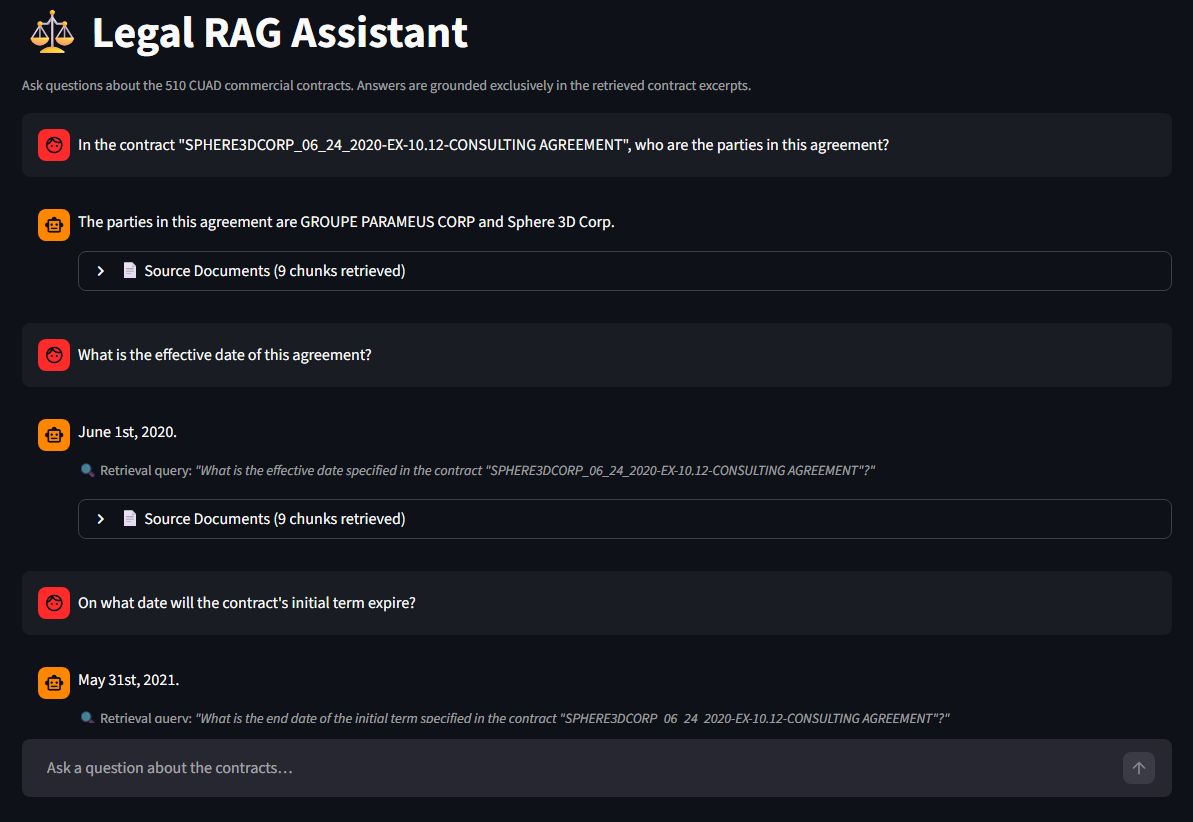
\includegraphics[width=\textwidth]{figures/memory1.png}
    \caption{Windowed memory session — questions 1 to 3.}
    \label{fig:memory1}
\end{figure}

\begin{figure}[h!]
    \centering
    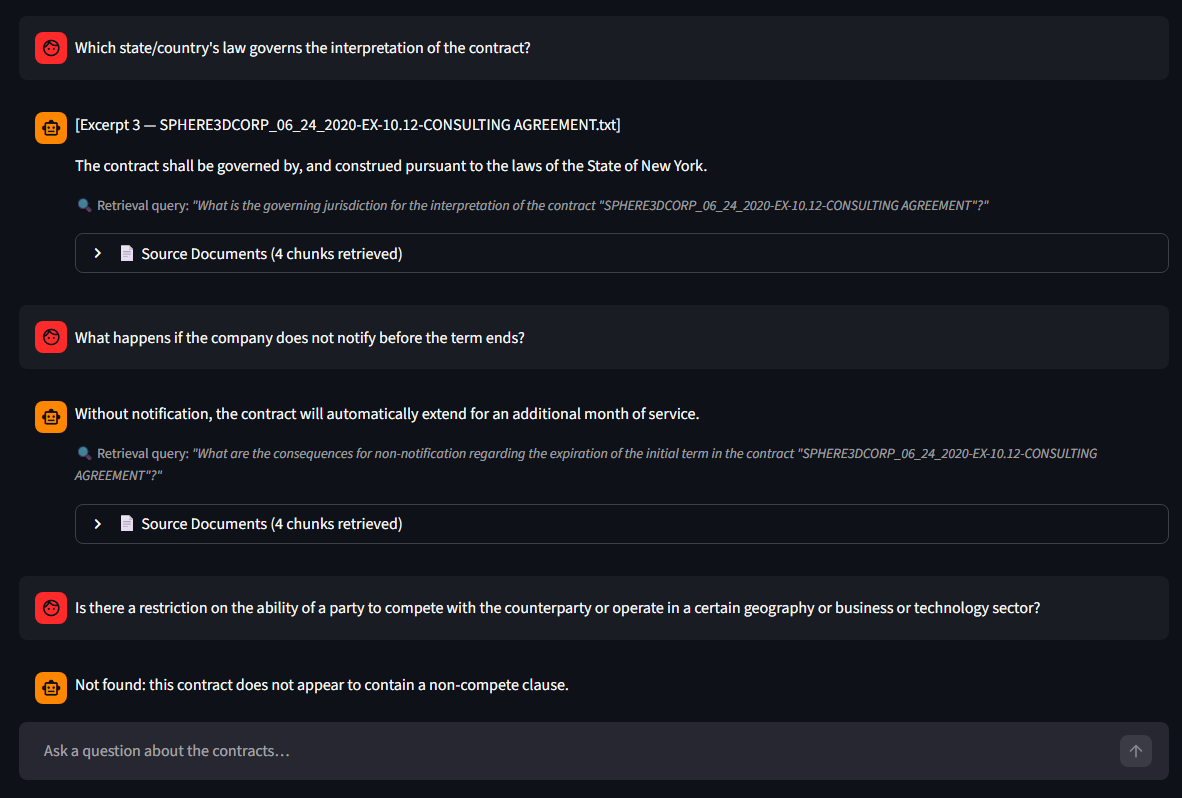
\includegraphics[width=\textwidth]{figures/memory2.png}
    \caption{Windowed memory session — questions 4 to 6.}
    \label{fig:memory2}
\end{figure}

\begin{figure}[h!]
    \centering
    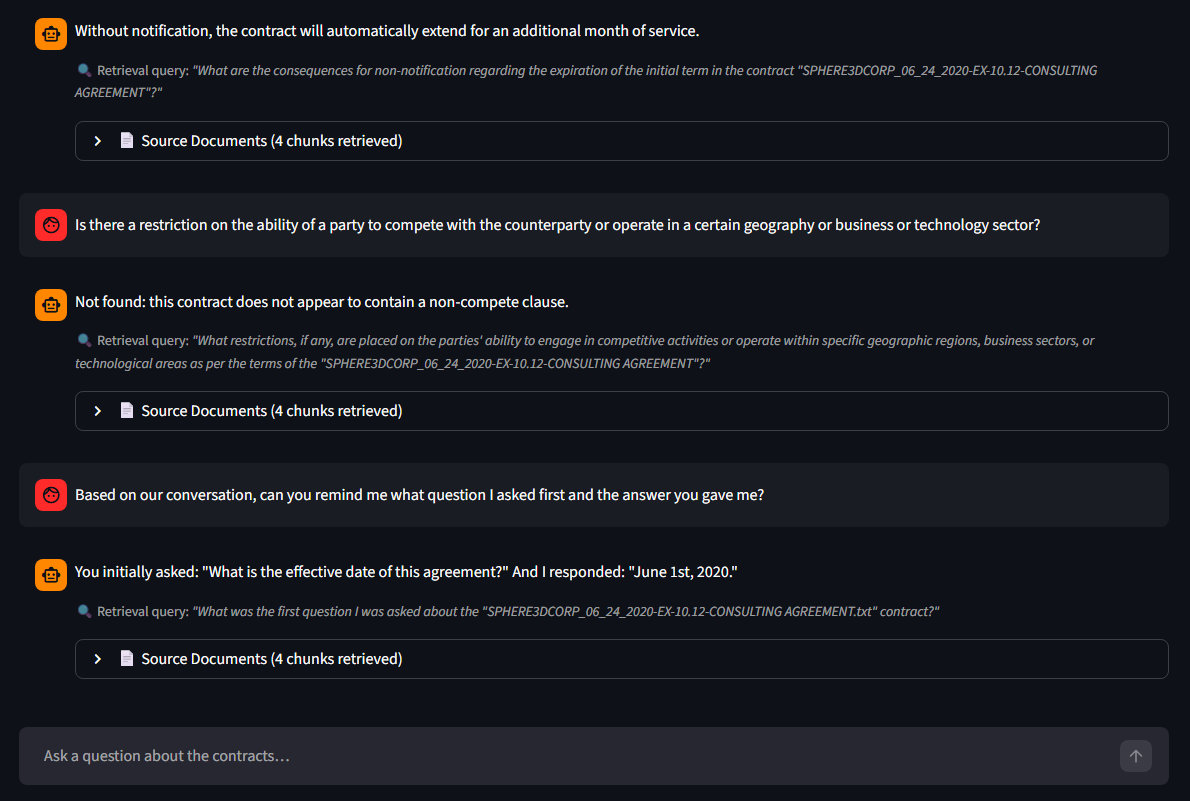
\includegraphics[width=\textwidth]{figures/memory3.png}
    \caption{Windowed memory failure at question 7. The model reports the effective date question as the first question asked, because question 1 (contracting parties) has been evicted from the $k=5$ window.}
    \label{fig:memory3}
\end{figure}

The failure appeared at question 7 (Figure~\ref{fig:memory3}). At that point the conversation history contained six completed turns. The windowed buffer holds only the last five, so question 1 — "In the contract SPHERE3DCORP\_06\_24\_2020-EX-10.12-CONSULTING AGREEMENT, who are the parties in this agreement?" — had been evicted from the context window. When asked to recall the first question of the session, the model identified question 2 ("What is the effective date of this agreement?") as the first, because that was the oldest turn still present in its window. The actual first question and its answer were permanently lost.

\newpage
\subsection{Summary Memory Results}

Under summary memory, the LLM maintains a running compressed summary of the full conversation after each turn. After question 1, the summary includes the fact that the user asked about the contracting parties and that the answer was GROUPE PARAMEUS CORP and Sphere 3D Corp. This summary is never truncated, it is updated incrementally and passed in full on every subsequent turn. When question 7 was asked under summary memory, the model correctly identified question 1 as the parties question and reproduced the correct answer, demonstrating that the information survived across all seven turns.

\begin{figure}[h!]
    \centering
    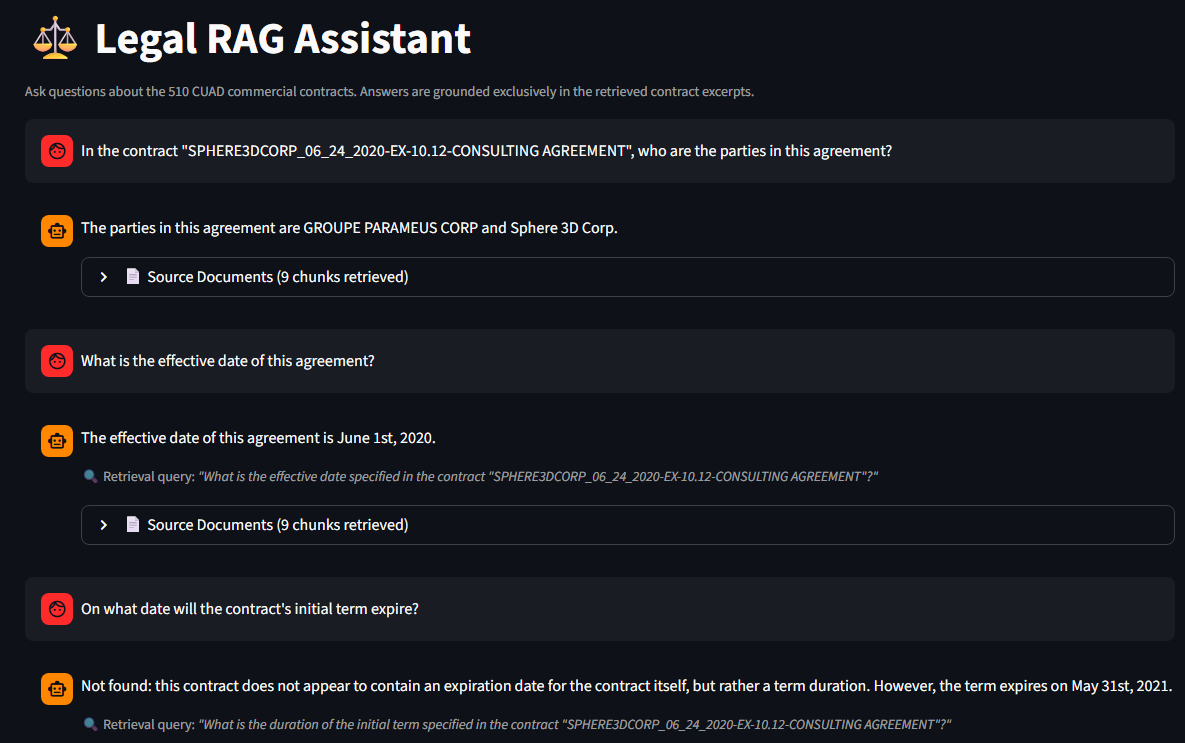
\includegraphics[width=\linewidth]{figures/summary1.png}
    \caption{Summary memory session — questions 1 to 3.}
    \label{fig:placeholder}
\end{figure}

\begin{figure}[h!]
    \centering
    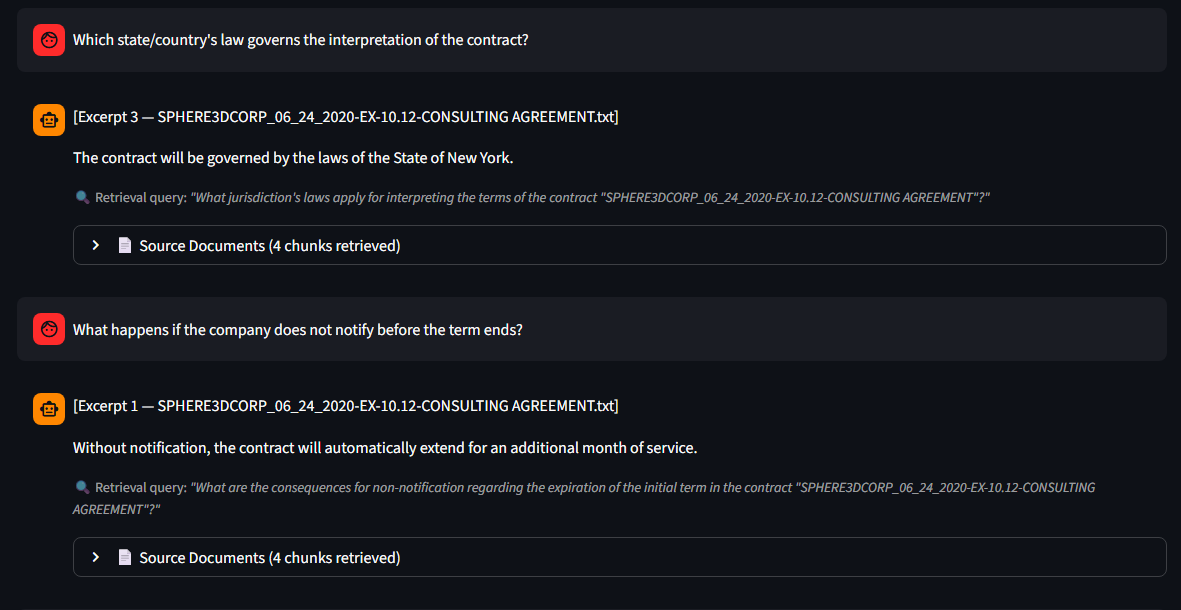
\includegraphics[width=\linewidth]{figures/summary2.png}
    \caption{Summary memory session — questions 4 to 5.}
    \label{fig:placeholder}
\end{figure}


\begin{figure}[h!]
    \centering
    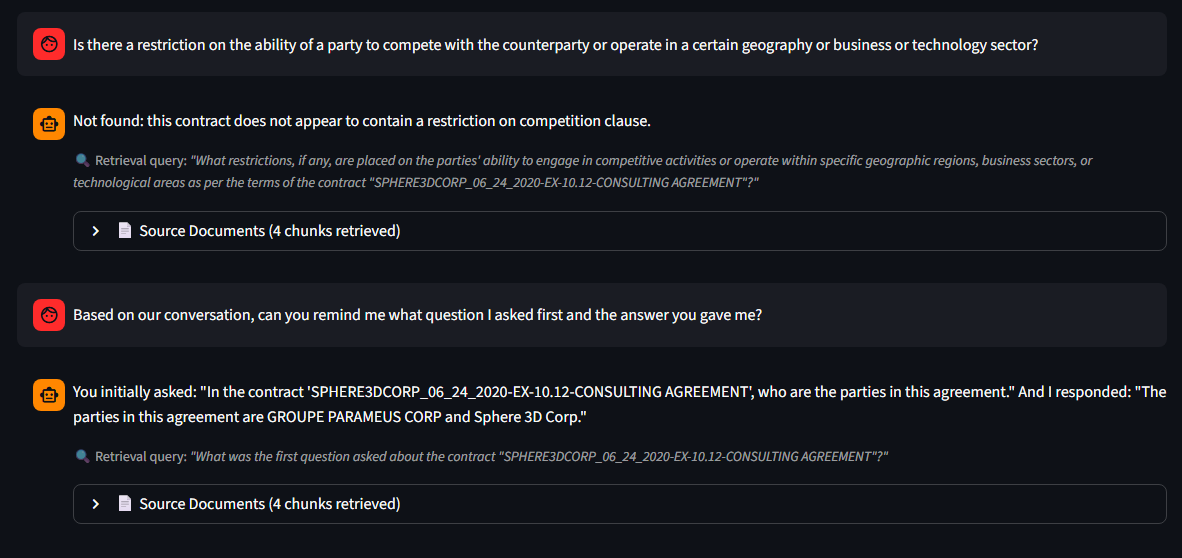
\includegraphics[width=1\linewidth]{figures/summary3.png}
    \caption{Summary memory session — questions 6 to 7.}
    \label{fig:placeholder}
\end{figure}

\newpage

\subsection{Discussion}

In a real case scenario, a user who wants to recall an earlier answer or question can simply scroll through the chat history in the interface. The test was done with this recall question to simply show the difference between the two memory window techniques. A more meaningful test is one where the model must retain context that the user stated about themselves, information that exists only in the conversation and cannot be retrieved from any document. To construct such a test, the first question of the session was modified to include a role declaration: "I am a lawyer representing the Consultant in this matter. In the contract SPHERE3DCORP\_06\_24\_2020-EX-10.12-CONSULTING AGREEMENT, who are the parties?". After five further questions covering the effective date, expiration, governing law, auto-renewal consequences, and non-compete restrictions, the seventh question asked: "Based on our conversation, which party am I representing, and what are their obligations if the company fails to give notice before the term ends?". This question cannot be answered by retrieval alone. The contract does not record who the user represents because that information exists only in Q1, which falls outside the windowed memory buffer at turn seven.

Under windowed memory (Figure ~\ref{fig:windowfinal}), the model answered "you are representing the company" it completely lost the context of the party, it didn't even provide the company name. Q1 had been evicted from the buffer after six turns, and the model had no record of the role declaration. With no grounded context to draw from, it guessed incorrectly. The condense chain also failed to reconstruct the contract filename, producing a vague retrieval query with no contract reference and retrieving ten chunks from multiple contracts.

\begin{figure}[h!]
    \centering
    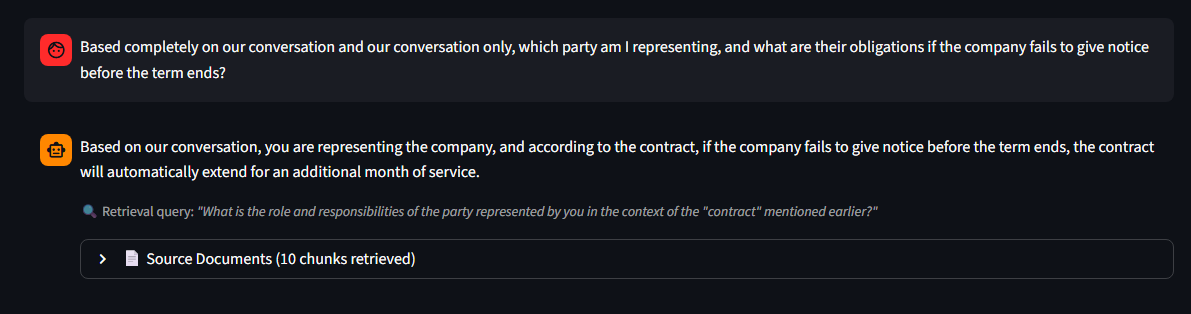
\includegraphics[width=\linewidth]{figures/windowfinal.png}
    \caption{Question 7 under windowed memory ($k=5$) — incorrect identification of the represented party.}
    \label{fig:windowfinal}
\end{figure}

Under summary memory (Figure ~\ref{fig:summaryfinal}), the model identified GROUPE PARAMEUS CORP as the party being represented and described the auto-extension clause as the relevant obligation. The role declaration from Q1 had been captured in the running summary and remained available throughout the session. The condense chain, informed by the richer summary, also generated a precise retrieval query that included the full contract filename, retrieving four targeted chunks rather than ten mixed ones. The phrase "based on our conversation only" was added deliberately to prevent the model from inferring the role from contract content, isolating memory as the only possible source of the answer.

\begin{figure}[h!]
    \centering
    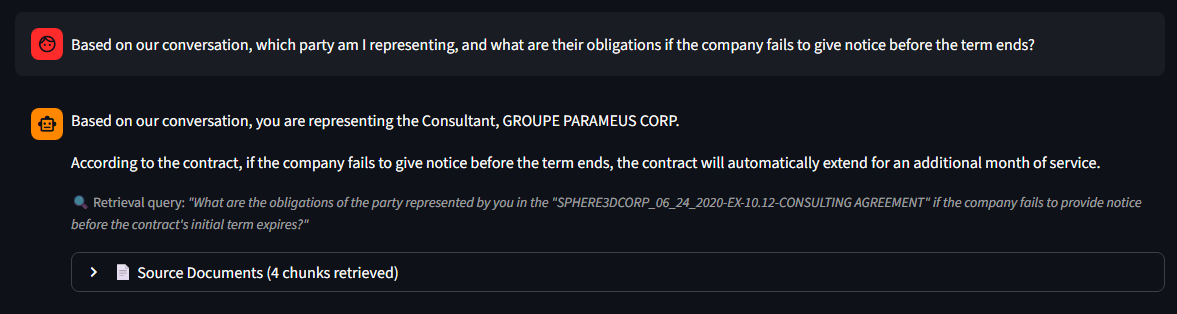
\includegraphics[width=\linewidth]{figures/summaryfinal.png}
    \caption{Question 7 under summary memory — correct identification of the consultant.}
    \label{fig:summaryfinal}
\end{figure}

Windowed memory is simple and guarantees exact verbatim recall of recent turns, but it silently discards older context once the buffer is full. Summary memory avoids this by compressing rather than discarding, at the cost of losing fine-grained verbatim detail in older turns. For long legal sessions that may span many clauses of a single contract, summary memory is the more appropriate choice, since a user may reference a clause discussed several turns earlier without the system having lost all trace of it.


